\chapter[Introducción a las Ecuaciones Diferenciales]{INTRODUCCIÓN A LAS ECUACIONES DIFERENCIALES}
\startcontents
\printchaptertableofcontents

En la Antigua Grecia, aunque no existía un cálculo formal, los matemáticos ya abordaban problemas complejos mediante procesos de aproximación. Un ejemplo emblemático es el método de \textit{exhausción} de Arquímedes. A pesar de carecer de la noción formal de límite, este enfoque anticipó de manera notable la idea moderna de aproximar el comportamiento de una función conforme se refina la partición, un concepto central en el análisis matemático.

El verdadero salto en el estudio de las ecuaciones diferenciales se produjo con la invención del cálculo por Isaac Newton y Gottfried Wilhelm Leibniz. Newton, a través de sus fluxiones, introdujo un lenguaje matemático para describir tasas de cambio, lo que le permitió formular sus leyes del movimiento y la gravitación. Estas ideas fueron esenciales para modelar el comportamiento dinámico de los cuerpos y establecer relaciones entre variables en movimiento. Por su parte, Leibniz desarrolló una notación más sistemática y simbólica, especialmente en lo que respecta a los diferenciales, lo que facilitó el tratamiento y la manipulación de estas expresiones en una gran variedad de problemas matemáticos. Así, se sentaron las bases para el estudio formal de las ecuaciones diferenciales.

Durante el siglo XVIII, el estudio de las ecuaciones diferenciales se vio enriquecido por las contribuciones de matemáticos como los hermanos Bernoulli, quienes aplicaron la técnica de separación de variables para resolver problemas surgidos tanto en la física como en la geometría. Leonhard Euler, uno de los matemáticos\infohyBulle{El método de exhausción consiste en aproximar el área o volumen de una figura compleja mediante una sucesión de figuras simples (como polígonos o prismas) que se ajustan cada vez mejor a la figura original. A medida que estas aproximaciones se refinan, se \textit{exhausta} la diferencia hasta alcanzar el valor exacto, anticipando el concepto moderno de límite.}
más prolíficos de la historia, sistematizó métodos para resolver ecuaciones de diversos órdenes y potenció el uso de series de potencias para obtener soluciones aproximadas en casos donde no era posible encontrar expresiones exactas. En este mismo periodo, se introdujeron las primeras ecuaciones no lineales mediante el trabajo de Riccati, y figuras como Lagrange y d’Alembert ampliaron el estudio de estas ecuaciones aplicando técnicas de variación de parámetros, lo que abrió la puerta a la solución de problemas más complejos y a la incorporación de nuevos métodos analíticos.

El siglo XIX marcó una etapa de consolidación y rigor en el campo. Augustin-Louis Cauchy estableció teoremas fundamentales de existencia y unicidad para problemas de valor inicial, lo cual permitió fundamentar la validez y la consistencia de las soluciones obtenidas. Posteriormente, matemáticos como Picard y Lindelöf perfeccionaron estos enfoques mediante métodos de aproximaciones sucesivas, ofreciendo herramientas más refinadas para tratar problemas donde la solución exacta era difícil de determinar. Además, figuras como Henri Poincaré y Aleksandr Lyapunov iniciaron el análisis cualitativo de las soluciones de ecuaciones diferenciales, centrándose en la estabilidad y el comportamiento a largo plazo de los sistemas dinámicos. Este análisis no solo enriqueció la teoría, sino que sentó las bases para áreas tan innovadoras como la teoría del caos.

En tiempos recientes, las ecuaciones diferenciales se han consolidado como herramientas esenciales en diversas ramas de la ciencia y la ingeniería. La combinación de métodos analíticos tradicionales—como la separación de variables y el uso de series de potencias—con técnicas numéricas modernas (por ejemplo, los métodos de Euler y Runge–Kutta) ha permitido modelar con gran precisión fenómenos en física, biología, economía e ingeniería. Esta integración de métodos teóricos y computacionales ha posibilitado la resolución de problemas complejos, desde la simulación de sistemas climáticos hasta la descripción de procesos biológicos, demostrando cómo la necesidad de resolver problemas prácticos impulsa continuamente el avance teórico en el estudio de las ecuaciones diferenciales.

\section{Conceptos Fundamentales}
Las ecuaciones diferenciales tienen una importancia fundamental en las matemáticas de la ingeniería, ya que permiten modelar de manera precisa la evolución y el comportamiento de sistemas físicos y geométricos a lo largo del tiempo y el espacio. Muchas leyes naturales, como las que rigen la transferencia de calor, el movimiento de fluidos, la dinámica de estructuras y la propagación de ondas, se expresan mediante relaciones que involucran tasas de cambio; es decir, mediante derivadas.

La capacidad para traducir un problema físico en un modelo matemático se ha convertido en una herramienta esencial en la ingeniería. Este proceso implica identificar las variables relevantes, establecer las relaciones entre ellas basadas en leyes físicas o principios geométricos, y finalmente expresar esas relaciones en forma de ecuaciones diferenciales. Una vez planteado el modelo, el análisis y la resolución de la ecuación—usando métodos analíticos como la separación de variables o series de potencias, o métodos numéricos como Euler y Runge–Kutta—permiten predecir el comportamiento del sistema y optimizar su desempeño.\sideFigure[\label{fig01}Esquema del problema físico que muestra a una persona caminando y jalando un bloque mediante una cuerda de longitud constante $L$. Se destacan la dirección del movimiento, la representación de la cuerda y el bloque, y el sistema de ejes que sitúa geométricamente los elementos.][1cm]{
    \begin{tikzpicture}[punteada/.style={thick,dash pattern=on 5pt off 4pt,gray},scale=0.82]
        \draw[punteada] (-0.4,0) -- (4,0);
        \draw[punteada] (0,-0.4) -- (0,0);
        \draw[punteada] (0,0.6) -- (0,4);
        %
        \draw[thick,-Stealth,red] (0.5,-0.5) -- (3.5,-0.5);
        \draw[thick,orange] (-0.6,0) -- node[midway, fill=white, inner sep=3pt] {\color{black}$L$} (-0.6,3);
        \foreach \y in {0,3} {
            \draw[thick,orange] (-0.7,\y) -- (-0.5,\y);
        }
        %
        \draw[thick,brown] (0,0.6) -- (0,3);
        % Cuerpo en movimiento
        \filldraw[fill=blue!20,draw=blue] (-0.25,2.75) rectangle (0.25,3.25);
        % Mono
        \node at (0,0.33) {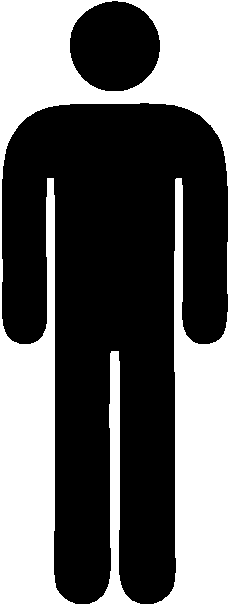
\includegraphics[scale=0.065]{images/capitulo1/fig1.pdf}};
    \end{tikzpicture}
}

En las siguientes líneas, presentaremos diversos ejemplos prácticos en los que se deducen las ecuaciones diferenciales a partir de situaciones reales. Este enfoque no solo ilustra el proceso de modelado matemático, sino que también subraya la estrecha relación entre la teoría y su aplicación en problemas de ingeniería. Es importante recordar que la transición del problema físico al modelo matemático es un pilar esencial en la ingeniería, ya que permite transformar datos y observaciones del mundo real en herramientas analíticas precisas y operativas.

\begin{example}{}{}
    Una persona camina en dirección horizontal jalando un bloque con una cuerda de una longitud constante $L$. Esta persona inicia un movimiento cuando la cuerda es ortogonal al eje horizontal. Vea la Figura \ref{fig01}.
    \begin{solucion}
        Como anteriormente mencionamos, este problema tiene por solución  un modelo matemático y nuestro primer objetivo será llevar la Figura \ref{fig01} a un sistema coordenado. De la siguiente forma:
        Donde $y(x)$ es la trayectoria que describe al bloque, $P(x,y)$\, es el punto tangencial a $\ell$, la cual es la recta que pasa por $P$\, y contiene a la cuerda (además, es tangente a $y(x)$). Note que la pendiente de $\ell$ es igual a $\theta$. De lo anterior, se sigue que
        \begin{equation}
            m_\ell = \tan (\theta). \label{ec01}
        \end{equation}
        Es decir,
        \begin{equation}
            m_\ell = \frac{d}{dx}y(x). \label{ec02}
        \end{equation}
        Entonces, de la ecuación \eqref{ec01} y de la ecuación \eqref{ec02} tenemos
        \begin{equation}
            \frac{d}{dx}y(x) = \tan (\theta). \label{ec03}
        \end{equation}
        Además, sabemos por la Figura \ref{fig02} que $\alpha + \theta = 180°$ o bien que $\alpha + \theta = \pi$. De lo anterior se sigue que $\theta = \pi - \alpha$. Ahora sustituimos en la ecuación \eqref{ec03} el valor de $\theta$
        \begin{align*}
            \frac{d}{dx}y(x) & = \tan (\pi - \alpha) \\
            & = \frac{\sen (\pi - \alpha)}{\cos (\pi - \alpha)}
            \intertext{Por identidades trigonométricas tenemos}
            & = \frac{\cancelto{0}{\sen(\pi}) \cdot \cos(\alpha) + \cos(\pi)\sen(-\alpha)}{\cos(\pi)\cos(-\alpha) - \cancelto{0}{\sen(\pi}) \cdot \sen(-\alpha)}
            \intertext{Por paridad del seno y coseno}
            & = -\frac{\cos(\pi)\sen(\alpha)}{\cos(\pi)\cos(\alpha)} \\
            & = -\frac{\sen(\alpha)}{\cos(\alpha)}.
        \end{align*}
        Por lo tanto,
        \begin{equation}
            \frac{d}{dx}y(x) = -\frac{\sen(\alpha)}{\cos(\alpha)}. \label{ec04}
        \end{equation}
        Luego, de la Figura \ref{fig02} note que
        \begin{equation} \label{ec05}
            \begin{aligned}
                \sen(\alpha) & = \frac{y}{L} \\
                \cos(\alpha) & = \frac{\sqrt{L^2 - y^2}}{L}
            \end{aligned}
        \end{equation}
        Sustituyendo a \eqref{ec05} en \eqref{ec04}
        \begin{align*}
            \frac{d}{dx}y(x) & = -\frac{\dfrac{y}{L}}{\dfrac{\sqrt{L^2 - y^2}}{L}}
        \end{align*}
        \begin{equation}
            \frac{d}{dx}y(x) + \frac{y}{\sqrt{L^2 - y^2}} = 0. \label{ec06}
        \end{equation}
        Para poder determinar la trayectoria del bloque, debemos de resolver la ecuación \eqref{ec06}.
    \end{solucion}
\end{example}
\sideFigure[\label{fig02}Representación del modelo matemático de la Figura \ref{fig01}. Se ilustra la trayectoria $y(x)$ del bloque, la recta tangente en el punto $P(x,y)$ y los ángulos involucrados, estableciendo la relación entre la derivada $\dfrac{dx}{dy}$ y la orientación de la cuerda.][-18cm]{
    \begin{tikzpicture}[scale=0.425,font=\tiny]
        %%%% Coordenadas. %%%%
        \coordinate (a) at (1.8,0);
        \coordinate (9) at (1.8,0.3);
        \coordinate (b) at (1.5,0.3);
        \coordinate (A) at (5.4,0);
        \coordinate (O) at (5.1855036855037,0);
        \coordinate (B) at (5.0191522822025,0.1354100422872);
        \coordinate (C) at (4.9710073710074,0);
        %%%%%% Ángulos. %%%%%%
        \draw[Aquamarine!70!black] (a) -- (9) -- (b);
        \draw pic["$\theta$",angle eccentricity=1.5,draw=Purple,angle radius=12,thick]{angle=A--O--B};
        \draw pic["$\alpha$",angle eccentricity=1.5,draw=Emerald,angle radius=12,thick]{angle=B--O--C};
        %%%%%% Función. %%%%%%
        \draw[domain=0:8,smooth,variable=\x,Green] plot ({\x}, {4.52-1.85*ln(\x+0.77)}) node[above] {\color{black}$y(x)$};
        %% Líneas del punto %%
        \draw[gray,dash pattern=on 3pt] plot [smooth] (1.5,0) -- (1.5,1.5) node[left] {\color{black}$y$} -- (1.5,3) -- (0,3);
        %%%%%% Eje x, y %%%%%%
        \draw[thick,-Stealth] (-0.4,0) -- (8,0) node[below] {$x$};
        \draw[thick,-Stealth] (0,-0.4) -- (0,6) node[left] {$y$};
        %%% Recta tangente %%%
        \draw[domain=-0.4:5.67690417,smooth,variable=\x,Dandelion] plot ({\x}, {3 - (1.85/2.27)*(\x-1.5)}) node[right] {\color{black}$\ell$};
        \node[below left] at (3.3405405405405,1.5) {$L$};
        %%%%%% Punto  P %%%%%%
        \filldraw[red] (1.5,3) circle (1pt) node[above right] {\color{black}$P(x,y)$};
        %%%%%%% Cuerpo %%%%%%%
        \filldraw[fill=blue!20,draw=blue] (-0.3,4.7) rectangle (0.3,5.3);
    \end{tikzpicture}
}En el ejemplo anterior hemos visto cómo, a partir de una situación física concreta, es posible obtener una ecuación diferencial que modela la trayectoria de un objeto en movimiento. Se identificaron las variables relevantes y se aplicaron principios geométricos para relacionarlas. Este mismo proceso de pasar de la situación real al modelo matemático es fundamental en la formulación de ecuaciones diferenciales. A continuación, analizaremos otro problema en el que, partiendo de un fenómeno epidemiológico, construiremos un modelo que describe la propagación de una enfermedad en una población. Notarás que, aunque los contextos sean distintos, la idea central de identificar interacciones y tasas de cambio se mantiene, demostrando la gran versatilidad de las ecuaciones diferenciales en la modelación de fenómenos diversos.

\begin{example}{}{}
    En una población aislada de $N$ habitantes, un individuo infectado entra a la población en el tiempo $t_0$. La enfermedad es contagiosa y se transmite mediante la interacción de los habitantes. \\
    \solucion Para un tiempo $t$, con $t > t_0$, sea $x(t)$ las personas contagiosas y $y(t)$ las personas no contagiadas. Vea la Figura \ref{fig03}. De lo cual se sigue $x(t) + y(t) = N + 1$, o bien, que
    \begin{equation}
        y(t) = N + 1 - x(t). \label{ec07}
    \end{equation}
    Además, sabemos que la tasa de crecimiento de las personas infectadas es \textbf{directamente proporcional} a la interacción entre las personas infectadas y las no infectadas. Dicha interacción se modela de la forma:
    $$x(t) \cdot y(t).$$
    La tasa de crecimiento esta dada por:
    \begin{equation}
        \frac{\Delta}{\Delta t}x(t) = k \cdot x(t) \cdot y(t), \, \text{con } \ k \in \RR^+. \label{ec08}
    \end{equation}
    Para la interpretación geométrica de lo anterior, vea la Figura \ref{fig04}.
    \begin{figure}
        \centering
        \begin{tikzpicture}
            %%%% Coordenadas. %%%%
            \coordinate (a) at (6.7,1);
            \coordinate (9) at (6.7,1.3);
            \coordinate (b) at (7,1.3);
            \coordinate (A) at (0.3,0);
            \coordinate (O) at (0,0);
            \coordinate (B) at (0.2683281573,0.13416407865);
            %%%%%% Ángulos. %%%%%%
            \draw pic["$\theta$",angle eccentricity=1.3,draw=Purple,angle radius=27,thick]{angle=A--O--B};
            \draw[Aquamarine!70!black,thick] (a) -- (9) -- (b);
            %% Líneas del punto %%
            \draw[gray,thick,dash pattern=on 3pt] plot [smooth] (2,0) -- (2,1);
            \draw[gray,thick,dash pattern=on 3pt] plot [smooth] (0,1) -- (2,1) -- (4.5,1) node[above] {\color{black}$\Delta x$} -- (7,1);
            \draw[gray,thick,dash pattern=on 3pt] plot [smooth] (7,0) -- (7,1) -- (7,2.25) node[right] {\color{black}$\Delta y$} -- (7,3.5) -- (0,3.5);
            %%%%%% Función. %%%%%%
            \draw[domain=0:8,smooth,variable=\x,Green,thick]
                plot ({\x}, {3.5^( (\x-2)/5 )})
                node[above right] {\color{black}$f(x)$};
            %%%%%%% Recta. %%%%%%%
            \draw[domain=0:8,smooth,variable=\x,orange,thick] plot ({\x}, {0.5*\x});
            %%%%%% Eje x, y %%%%%%
            \draw[very thick,-Stealth] (-0.4,0) -- (8,0) node[below] {$x$};
            \draw[very thick,-Stealth] (0,-0.4) -- (0,5) node[left] {$y$};
            \foreach \y [count=\i] in {1,3.5} {
                \draw[very thick] (0,\y) -- (-0.15,\y) node[left] {$y_{\i}$};
            }
            \foreach \x [count=\i] in {2,7} {
                \draw[very thick] (\x,0) -- (\x,-0.15) node[below] {$x_{\i}$};
            }
            %%%%%% Puntos. %%%%%%
            \filldraw[red] (2,1) circle (1.5pt) node[above left] {\color{black}$(x_1,y_1)$};
            \filldraw[red] (7,1) circle (1.5pt) node[right] {\color{black}$(x_2,y_1)$};
            \filldraw[red] (7,3.5) circle (1.5pt) node[right] {\color{black}$(x_2,y_2)$};
        \end{tikzpicture}
        \caption{Gráfica explicativa del proceso de modelado en el problema de contagio. Muestra cómo los incrementos $\Delta x$ y $\Delta y$ se relacionan con la tasa de cambio (derivada), facilitando la interpretación geométrica del modelo diferencial que describe la propagación del contagio.}
        \label{fig04}
    \end{figure}
    Ahora de la ecuación \eqref{ec08}, cuando $\Delta t \to 0$ tenemos
    $$\frac{\Delta}{\Delta t}x(t) \xrightarrow[\Delta t \to 0]{} \frac{d}{d(t)}x(t) \quad \text{o bien} \quad \lim_{\Delta t \to 0} \frac{\Delta}{\Delta t}x(t) = \frac{d}{dt}x(t).$$
    Ahora, se sigue que
    \begin{align}
        k \cdot x(t) \cdot y(t) & = \lim_{\Delta t \to 0} \frac{\Delta}{\Delta t}x(t) = \frac{d}{dt}x(t) \nonumber \\
        \frac{d}{dt}x(t) & = k \cdot x(t) \cdot y(t). \label{ec09}
    \end{align}
    Sustituyendo la expresión \eqref{ec07} en la ecuación \eqref{ec09}
    \begin{align}
        \frac{d}{dt}x(t) & = k \cdot x(t) \cdot y(t) \nonumber \\
        \frac{d}{dt}x(t) - k \cdot x(t) \cdot y(t) & = 0 \label{ec10}
    \end{align}
    Para poder hallar a $f(x)$ (la función que describe el índice de contagios), es necesario resolver la ecuación \eqref{ec10}.
\end{example}
Entre estos dos ejemplos podemos apreciar que, aunque los contextos sean muy diferentes—uno aborda la dinámica de un objeto en movimiento y el otro la propagación de una enfermedad—el proceso de pasar de una situación real a un modelo matemático es esencial en la ingeniería. En ambos casos se identifican las variables críticas, se establecen relaciones a través de tasas de cambio y se llega a una ecuación diferencial que captura la esencia del fenómeno.

Esta capacidad de abstracción y modelado diferencial es lo que permite aplicar estos métodos en contextos tan variados. De hecho, a continuación veremos cómo se emplea el mismo enfoque para resolver un problema en el campo de la óptica: el diseño de un espejo que concentre los rayos solares en un único punto. Este siguiente ejemplo ilustra que, independientemente del área—ya sea mecánica, epidemiológica u óptica—las ecuaciones diferenciales constituyen una herramienta fundamental para entender y optimizar sistemas complejos.

\begin{example}{}{}
    Se requiere determinar la forma de un espejo, que concentre los rayos del Sol es un solo punto, para el aprovechamineto de la energía solar. Vea la Figura \ref{fig05}.
    \begin{figure}
        \centering
        \begin{tikzpicture}
            %%%% Coordenadas. %%%%
            \coordinate (a) at (2.7,0);
            \coordinate (9) at (2.7,0.3);
            \coordinate (b) at (3,0.3);
            \coordinate (O1) at (0,0);
            \coordinate (A1) at (0.2,0);
            \coordinate (B1) at (0.1414213562372,0.1414213562372);
            %
            \coordinate (O2) at (3,3);
            \coordinate (A2) at (3,2.7);
            \coordinate (B2) at (2.787867965644,2.787867965644);
            %
            \coordinate (A3) at (2.7,3);
            \coordinate (B3) at (2.8289467290207,3.2464564433877);
            %
            \coordinate (O4) at (5,0);
            \coordinate (A4) at (4.7,0);
            \coordinate (B4) at (4.8335899411324,0.2496150883014);
            %
            \coordinate (A5) at (5.3,0);
            %%%%%% Ángulos. %%%%%%
            \draw pic["$\delta$",angle eccentricity=1.4,draw=Purple,angle radius=15,thick]{angle=A1--O1--B1};
            %
            \draw[Aquamarine!70!black,thick] (a) -- (9) -- (b);
            \draw pic["$\alpha$",angle eccentricity=1.35,draw=Purple,angle radius=15,thick]{angle=B2--O2--A2};
            %
            \draw pic["$\alpha$",angle eccentricity=1.35,draw=Purple,angle radius=15,thick]{angle=B3--O2--A3};
            %
            \draw pic["$\alpha$",angle eccentricity=1.35,draw=Purple,angle radius=15,thick]{angle=B4--O4--A4};
            %
            \draw pic["$\theta$",angle eccentricity=1.35,draw=BlueGreen,angle radius=15,thick]{angle=A5--O4--B4};
            %%%%%% Eje x, y %%%%%%
            \draw[very thick,-Stealth] (-4,0) -- (6,0) node[below] {$x$};
            \draw[very thick,-Stealth] (0,-4) -- (0,4) node[left] {$y$};
            %%%%%% Función. %%%%%%
            \draw[thick,Green] plot[domain=4:-4,samples=100] ({4 - (\x*\x)/9}, {\x}) node[below right] {\color{black}$y(x)$};
            %%% Recta tangente %%%
            \draw[domain=2.3333333333333:6,smooth,variable=\x,Dandelion,thick] plot ({\x}, {-3/2*\x + 15/2}) node[right] {\color{black}$\ell$};
            %%%%%% Cuadrado %%%%%%
            \draw[thick,blue] (-3,3) -- (3,-3);
            \draw[thick,blue] (-3,-3) -- (0,0);
            \filldraw[fill=none,draw=gray,thick,dash pattern=on 4pt] (-3,-3) rectangle (3,3);
            \draw[thick,Orange!50!Red] (0,0) -- (1.5,1.5) node[above,rotate=45] {\color{black}$\sqrt{x^2 + y^2}$} -- (3,3);
            %%%%%%% Puntos %%%%%%%
            \filldraw[BrickRed] (3,3) circle (1.5pt) node[right] {\color{black}$P(x,y)$};
            \filldraw[BlueViolet] (5,0) circle (1.5pt) node[below left] {\color{black}$Q$};
            \node[below left] at (3,0) {$x_1$};
            \node[above left] at (0,3) {$y_1$};
        \end{tikzpicture}
        \caption{La figura ilustra la configuración geométrica para diseñar un espejo que concentra los rayos solares en un punto. Se muestra la curva $y(x)$, el punto de reflexión $P(x,y)$ con su tangente, y se indican los ángulos $\delta$ y $\alpha$ que permiten establecer las relaciones trigonométricas fundamentales para deducir la ecuación diferencial del modelo.}
        \label{fig05}
    \end{figure}
    \solucion Sea $y(x)$ la forma del espejo y sea $P$ un punto cualquiera de la curva $y(x)$. Entonces el ángulo de indiferencia es igual al ángulo de reflexión $\alpha$. Ahora, el triángulo $(P \,\, O \, Q)$ tiene a $\theta$ como un ángulo externo. Así
    \begin{equation}
        \theta = \delta + \alpha. \label{ec11}
    \end{equation}
    Además
    \begin{align}
        \theta + \alpha & = 180° \nonumber \\
        \theta + \alpha & = \pi. \label{ec12}
    \end{align}
    De las ecuaciones \eqref{ec11} y \eqref{ec12} se sigue que
    \begin{equation}
        \delta + 2\alpha = \pi. \label{ec13}
    \end{equation}
    Observe que $\ell$ es la recta tangente a $y(x)$ en el punto $P$. De lo cual, se sigue que
    \begin{align*}
        m_\ell & = \tan(\theta) = y'(x) \\
        \frac{d}{dx}y(x) & = \tan(\theta).
    \end{align*}
    Despejando a $\theta$ de la ecuación \eqref{ec12} y sustituyendo en lo anterior, tenemos
    \begin{equation}
        \frac{d}{dx}y(x) = \tan(\pi - \alpha) = \frac{\sen(\pi - \alpha)}{\cos(\pi - \alpha)} \label{ec14}
    \end{equation}
    De la expresión \eqref{ec13} obtenemos
    \begin{equation*}
        \alpha = \frac{\pi}{2} - \frac{\delta}{2}
    \end{equation*}
    Sustituyendo esto último en la ecuación \eqref{ec14}
    \begin{align*}
        \frac{d}{dx}y(x) & = \frac{\sen\left(\pi - \left(\dfrac{\pi}{2} - \dfrac{\delta}{2}\right)\right)}{\cos\left(\pi - \left(\dfrac{\pi}{2} - \dfrac{\delta}{2}\right)\right)} \\
        & = \frac{\sen\left(\dfrac{\pi}{2} + \dfrac{\delta}{2}\right)}{\cos\left(\dfrac{\pi}{2} + \dfrac{\delta}{2}\right)} \\
        & = \frac{\sen\left(\dfrac{\pi}{2}\right)\cos\left(\dfrac{\delta}{2}\right) + \cos\left(\dfrac{\pi}{2}\right)\sen\left(\dfrac{\delta}{2}\right)}{\cos\left(\dfrac{\pi}{2}\right)\cos\left(\dfrac{\delta}{2}\right) - \sen\left(\dfrac{\pi}{2}\right)\sen\left(\dfrac{\delta}{2}\right)} \\
        & = \frac{\cos\left(\dfrac{\delta}{2}\right)}{-\sen\left(\dfrac{\delta}{2}\right)}.
    \end{align*}
    Por lo tanto, tenemos que
    \begin{equation}
        \frac{d}{dx}y(x) = -\frac{\cos\left(\dfrac{\delta}{2}\right)}{\sen\left(\dfrac{\delta}{2}\right)}. \label{ec15}
    \end{equation}
    Recordemos que
    \begin{align*}
        \cos^2(A) & = \frac{1 + \cos(2A)}{2} \qquad & \sen^2(2A) & = \frac{1 - \sen(2A)}{2}
        \intertext{Sea $A = \dfrac{\delta}{2}$, entonces}
        \cos^2\left(\frac{\delta}{2}\right) & = \frac{1 + \cos(\delta)}{2} \qquad & \sen^2\left(\frac{\delta}{2}\right) & = \frac{1 - \sen(2A)}{2} \\
        \cos(\delta) & = \sqrt{\frac{1 + \cos(\delta)}{2}} \qquad & \sen(\delta) & = \sqrt{\frac{1 - \sen(\delta)}{2}}
    \end{align*}
    Sustituyendo estos últimos resultados en la ecuación \eqref{ec15}
    \begin{align*}
        \frac{d}{dx}y(x) & = -\frac{\sqrt{\dfrac{1 + \cos(\delta)}{2}}}{\sqrt{\dfrac{1 - \sen(\delta)}{2}}} \\
        & = -\sqrt{\frac{\dfrac{1 + \cos(\delta)}{2}\,}{\dfrac{1 - \cos(\delta)}{2}}} \\
        & = -\sqrt{\frac{1 + \cos(\delta)}{1 - \cos(\delta)}} \\
        & = -\sqrt{\frac{(1 + \cos^2(\delta))^2}{(1 - \cos(\delta))(1 + \cos(\delta))}} \\
        & = -\sqrt{\frac{(1 + \cos(\delta))^2}{1 + \cos^2(\delta)}} \\
        & = -\sqrt{\frac{(1 + \cos(\delta))^2}{\sen^2(\delta)}}.
    \end{align*}
    Por lo tanto,
    \begin{equation}
        \frac{d}{dx}y(x) = -\sqrt{\frac{(1 + \cos(\delta))^2}{\sen^2(\delta)}}. \label{ec16}
    \end{equation}
    Luego,  de la Figura \ref{fig05} vemos que
    \begin{equation} \label{ec17}
        \begin{aligned}
            \sen(\delta) & = \frac{y}{\sqrt{x^2 + y^2}} \\
            \cos(\delta) & = \frac{x}{\sqrt{x^2 + y^2}}
        \end{aligned}
    \end{equation}
    Sustituyendo la ecuación \eqref{ec17} en la ecuación \eqref{ec16}
    \begin{equation*}
        \frac{d}{dx}y(x) = -\frac{1 + \dfrac{x}{\sqrt{x^2 + y^2}}}{\dfrac{y}{\sqrt{x^2 + y^2}}} = -\frac{\dfrac{\sqrt{x^+ y^2} + x}{\sqrt{x^2 + y^2}}}{\dfrac{y}{\sqrt{x^2 + y^2}}} = -\frac{\sqrt{x^2 + y^2} + x}{y}.
    \end{equation*}
    Por lo tanto, obtenemos que
    \begin{equation}
        \frac{d}{dx}y(x) + \frac{\sqrt{x^2 + y^2} + x}{y} = 0.\label{ec18}
    \end{equation}
    De esta forma, para hallar la forma de la ecuación para formar el espejo ($y(x)$), tenemos que resolver la ecuación \eqref{ec18}.
\end{example}
Los ejemplos anteriores han ilustrado cómo, mediante la identificación de variables clave y el análisis de las relaciones entre ellas, es posible traducir situaciones reales—ya sea el movimiento de un objeto, la propagación de una enfermedad o el diseño óptico—en modelos matemáticos basados en ecuaciones diferenciales. Entre estos casos se aprecia que, aunque los contextos sean muy distintos, el proceso de transformar una situación del mundo real en un modelo matemático es esencial en la ingeniería: se identifican las variables críticas, se establecen relaciones a través de tasas de cambio y se llega a una ecuación diferencial que captura la esencia del fenómeno.

Esta capacidad de abstracción y modelado diferencial permite aplicar estos métodos en contextos tan variados. De hecho, en el ámbito de la electricidad se\sideFigure[\label{fig06}La \textbf{Ley de Kirchhoff} nos dicta que el voltaje $\varepsilon(t)$ es la suma de los voltajes en cada elemento del circuito LCR.]{
    \begin{circuitikz}[american,scale=0.55]
        \draw (0,0) to[C, l=$C$] (-4,0)
            to[sV, v=$\varepsilon(t)$] (-4,4)
            to[cute inductor, l=$L$] (0,4)
            to[R, l=$R$] (0,0);
        \draw[-latex] (-3.8,2.95) arc(180:90:8.5mm) node[midway,inner sep=1pt,fill=white] {\tiny$i(t)$};
    \end{circuitikz}
}
aplica el mismo principio. La Ley de Kirchhoff, por ejemplo, nos dicta que el voltaje total en un circuito es igual a la suma de los voltajes en cada uno de sus componentes. Esta relación se traduce en una ecuación diferencial que describe la evolución de la corriente $i(t)$ en un circuito LRC.

A continuación, abrimos paso a un ejemplo práctico con un circuito LRC.

\begin{example}{}{}
    Considere el circuito LRC de la Figura \ref{fig06}. Determine $i(t)$. \\
    \solucion En la inductancia ($L$), el voltaje está dado por:
    \begin{align*}
        L \cdot \frac{d}{dt}i(t) && \text{(las unidades de $L$ son los henrios ($H$))}
    \end{align*}
    En la resistencia ($R$), el voltaje está dado por
    \begin{align*}
        R \cdot i(t) && \text{(las unidades de $R$ son los ohmios ($\Omega$))}
    \end{align*}
    En el capacitor ($C$), el voltaje está dado por
    \begin{align*}
        \frac{1}{c} \int_0^1 i(\tau) \, d\tau && \text{(las unidades de $C$ son los faradios ($F$))}
    \end{align*}
    De lo cual, se sigue que
    \begin{equation}
        \varepsilon(t) = L \cdot \frac{d}{dt}i(t) + R \cdot i(t) + \frac{1}{c} \int_0^1 i(\tau) \, d\tau
    \end{equation}
    Por lo tanto, hemos determinado a $i(t)$.
\end{example}
\infoBulle{$\displaystyle i(t) = \frac{d}{dt}q(t)$, donde a $q$ se le llama carga y $L$, $R$ y $C$ son constantes.}

Los ejemplos presentados demuestran claramente cómo la formulación de problemas reales—ya sea en el contexto del movimiento, la propagación de contagios, el diseño óptico o el análisis de circuitos eléctricos—se puede traducir en modelos matemáticos que capturan la dinámica esencial de cada fenómeno. La capacidad para expresar estas relaciones en términos de derivadas y tasas de cambio es lo que hace de las ecuaciones diferenciales una herramienta indispensable en la ingeniería y las ciencias.

Para formalizar este enfoque y establecer una base teórica sólida, es importante definir qué entendemos por ecuación diferencial y, en particular, qué implica una ecuación diferencial ordinaria (EDO). A continuación, presentamos dos definiciones fundamentales que servirán de marco para el estudio y la aplicación de estos modelos.
\begin{definition}{}{}
    Una \textbf{ecuación diferencial} es una ecuación que contiene una o más derivadas de una o más variables dependientes respecto de una o más variables independientes.
\end{definition}

\begin{definition}{}{}
    Se le denomina \textbf{ecuación diferencial ordinaria} (por simplicidad, en el resto del texto les denominaremos \textbf{EDO}) a la ecuación diferencial que contiene una o más derivadas de una o más variables dependientes respecto a \textbf{una sola} variable independiente.
\end{definition}